\section{Real-data results and comparisons}
\subsection{One held-out trajectory and its fitted jerk}
Figure~\ref{fig:forecast} shows a predeclared chronological cutoff of the first real US-101 vehicle segment. The original recorded positions, smooth in-sample trend and extrapolated future are shown separately. Predictions are made without seeing the future; the PLS fit itself contains no built-in forecast model.
\begin{figure*}[t]\centering
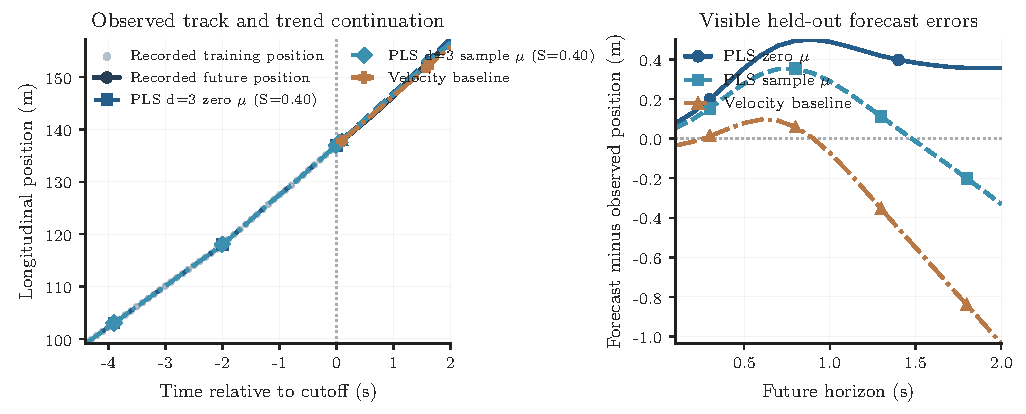
\includegraphics[width=\textwidth]{figures/heldout_forecast.pdf}
\caption{Measured training and future longitudinal position, with $d=3$ GCV-selected PLS trends under zero and training-derived means and their local-polynomial continuations. The observed future is withheld during estimation.}
\label{fig:forecast}
\end{figure*}
Third differences have meaningful units only after dividing by the cubed 0.1-s sampling interval. Figure~\ref{fig:jerk} illustrates strong differentiation noise in the original position and the smaller, regularized jerk proxy of the selected PLS trend. Neither derivative is independently observed true jerk.
\begin{figure*}[t]\centering
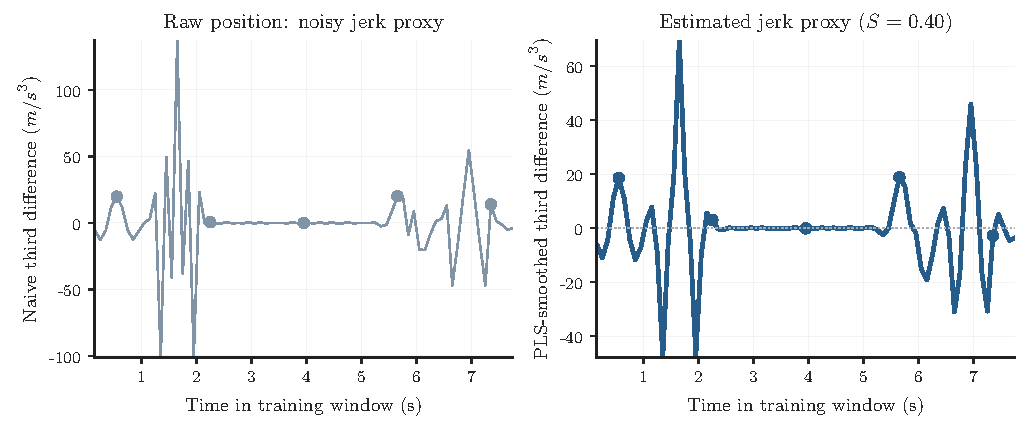
\includegraphics[width=\textwidth]{figures/jerk_comparison.pdf}
\caption{Direct and PLS-smoothed third differences of the same measured US-101 position segment. Panel axes have different scales; reduced amplitude after smoothing does not establish physical accuracy.}
\label{fig:jerk}
\end{figure*}

\subsection{Five criteria, four orders and both mean policies}
Table~\ref{tab:forecast} reports genuinely held-out position RMSE at the one-second horizon for the main PLS orders and physical baselines; Figure~\ref{fig:criteria} provides the complete $d=1,\ldots,4$ by five-criterion comparison for both $\mu=0$ and training-data plug-in mean of differences. Every method is scored against the same recorded future positions, not an unavailable noise-free latent trend.
% GENERATED FROM REAL NGSIM HOLDOUT RESULTS; DO NOT EDIT
\begin{table*}[t]
\caption{Out-of-sample position RMSE in meters at a one-second horizon (15 chronological track-origin windows). The five selection criteria used the same normalized S candidates, except restricted BIC ($S\ge0.10$). The data-derived mean policy changes model specification and does not yield exact refitted LOOCV.}
\label{tab:forecast}\centering
\begin{tabular}{lrrrr}
\toprule
Selector & $d=2,\ \mu=0$ & $d=3,\ \mu=0$ & $d=3,\ \widehat\mu$ & $d=4,\ \mu=0$ \\
\midrule
CV & 0.600 & 0.583 & 0.475 & 0.933 \\
GCV & 0.600 & 0.583 & 0.475 & 0.933 \\
AICc & 0.600 & 0.583 & 0.475 & 0.932 \\
Restricted BIC & 0.600 & 0.583 & 0.475 & 0.933 \\
Profile ML & 0.600 & 0.583 & 0.475 & 0.932 \\
\midrule
Velocity baseline & \multicolumn{4}{c}{0.547} \\
Acceleration baseline & \multicolumn{4}{c}{0.626} \\
Savitzky--Golay velocity & \multicolumn{4}{c}{0.543} \\
\bottomrule
\end{tabular}
\end{table*}

% AUTO-GENERATED REAL-DATA RESULTS
For $d=3$, GCV-selected PLS continued from 80 observed frames gives
0.583\,m RMSE under fixed $\mu=0$ and 0.475\,m
when the training-only sample mean of third differences is plugged in.
The corresponding constant-velocity and constant-acceleration baselines
give 0.547\,m and
0.626\,m, respectively.
The comparison is illustrative; highly similar criterion-level scores
do not indicate five independent demonstrations of superiority.

\begin{figure*}[t]\centering
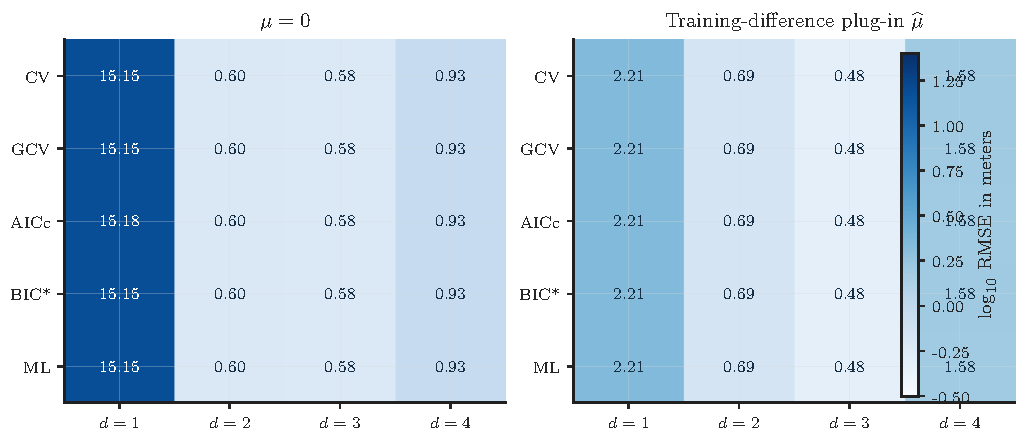
\includegraphics[width=\textwidth]{figures/criterion_heatmap.pdf}
\caption{Held-out one-second position RMSE in meters (printed values) across all four orders and all five criteria; $\mu$ policies are separated. Colors represent log-RMSE for display, not significance. BIC was restricted to $S\ge0.10$.}
\label{fig:criteria}
\end{figure*}

\subsection{Extrapolation horizon and physical baselines}
The experiment evaluates $h=5,10,20$ future 100-ms frames rather than labeling in-sample fitted values as forecasts. Figure~\ref{fig:horizons} compares selected $d=2,d=3$ PLS continuations with constant-velocity, constant-acceleration and Savitzky--Golay physical baselines. Smooth historical fits can extrapolate poorly if acceleration changes abruptly.
\begin{figure*}[t]\centering
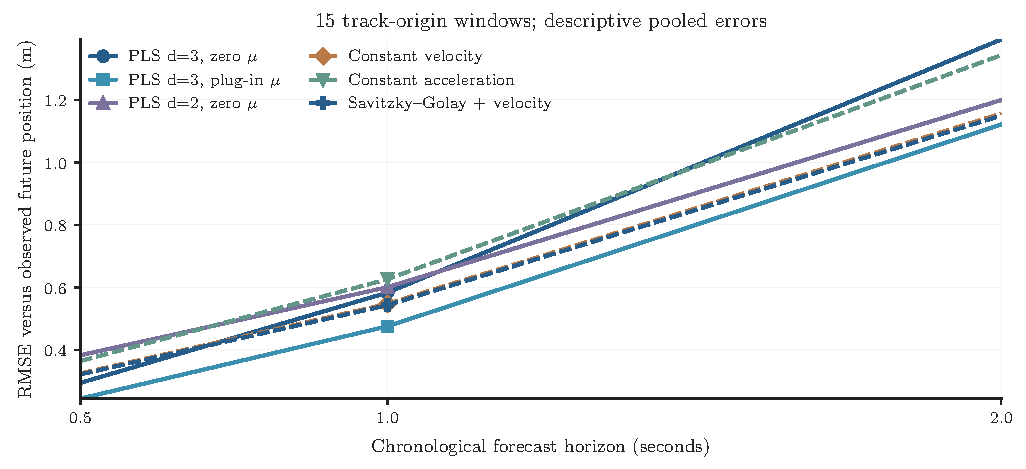
\includegraphics[width=\textwidth]{figures/forecast_horizons.pdf}
\caption{Chronological 0.5, 1 and 2-second position errors across 15 overlapping track-origin windows; comparisons use future measured camera-derived position, not latent truth.}
\label{fig:horizons}
\end{figure*}

\subsection{All seven numerical fitting pathways}
For completeness, we separately compare shift-free full SVD, dense solve, dense Cholesky, general banded LU, banded Cholesky, symmetric Gram eigendecomposition and dual SVD using the same observed windows at $d=3,S=0.9$. Table~\ref{tab:solver} and Figure~\ref{fig:backend} give fit-only median timings and relative fit discrepancies against SVD. This is a numerical calculation study, not a five-criterion selection runtime study or a measurement of physical jerk accuracy.
% GENERATED FROM REAL NGSIM FITTING BENCHMARK
\begin{table*}[t]
\caption{Same observed position windows, seven fit-only numerical backends, $d=3$, $S=0.90$. Median runtime is across 10 model/mean cases, each with three within-run timing repetitions; maximum relative fit error uses full SVD as the numerical baseline. Hardware-specific values do not predict criterion-selection timing.}
\label{tab:solver}\centering
\begin{tabular}{lrrr}\toprule
Solver & Valid cases & Median fit time (ms) & Max.\ relative discrepancy \\
\midrule
Full SVD & 10 & 0.0423 & 0.00e+00 \\
Dense LU & 10 & 0.0566 & 1.38e-12 \\
Dense Cholesky & 10 & 0.0401 & 1.65e-12 \\
Banded LU & 10 & 0.2047 & 1.27e-12 \\
Banded Cholesky & 10 & 0.0192 & 1.07e-12 \\
Gram eigendecomp. & 10 & 0.4226 & 3.26e-12 \\
Dual SVD & 10 & 0.6657 & 2.62e-17 \\
\bottomrule
\end{tabular}
\end{table*}

\begin{figure*}[t]\centering
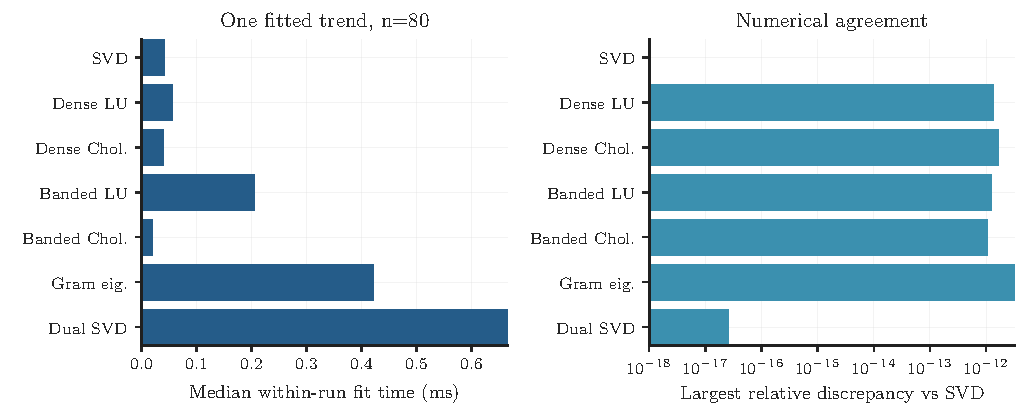
\includegraphics[width=\textwidth]{figures/backend_comparison.pdf}
\caption{Fit-only elapsed milliseconds and relative numerical discrepancies on real recorded positions under two $\mu$ policies. Numerical fit differences are not statistical forecast errors.}
\label{fig:backend}
\end{figure*}
